\documentclass[a4paper,12pt,twoside,openright]{article}
\usepackage[titletoc]{appendix}
\usepackage{textcomp}
\usepackage[pdftex]{color,graphics}
\usepackage{amssymb}
\usepackage{verbatim}
\usepackage{graphicx}
\usepackage{graphics}
\usepackage{amsmath}
\usepackage{rotating}
\usepackage{setspace}
\usepackage{multirow}
\usepackage{array}
\usepackage{hhline}
\usepackage[labelfont={bf}, margin=0.5cm]{caption}
\usepackage{pdflscape}
\usepackage{subcaption}
\usepackage{caption}
\usepackage{xspace}
\usepackage{float}
\usepackage{placeins}
\usepackage{etoolbox}
\usepackage{xkeyval}[2006/11/18]
\usepackage{datetime}
\usepackage[a4paper,inner=1.5cm,outer=1.5cm,top=2.5cm,bottom=2.5cm,pdftex]{geometry}
\usepackage{emptypage}
\usepackage{hyperref}

\hypersetup{
	linktocpage,
    colorlinks = true,
	linkcolor = blue,
	citecolor = red
}

\usepackage{fancyhdr}
\fancyfoot{}
\pagestyle{fancy}
\fancyhead[LO]{\leftmark}
\fancyhead[RE]{\rightmark}
\fancyhead[RO,LE]{\thepage}

\renewcommand{\textfraction}{.05}
\renewcommand{\floatpagefraction}{.40}

\newcommand{\gr}{$\gamma$-ray\xspace}
\newcommand{\grs}{$\gamma$-rays\xspace}

\usepackage{lipsum}% just to automatically generate text

\makeatletter
\newcommand\ackname{Acknowledgements}
\if@titlepage
  \newenvironment{acknowledgements}{%
      \titlepage
      \null\vfil
      \@beginparpenalty\@lowpenalty
      \begin{center}%
        \bfseries \ackname
        \@endparpenalty\@M
      \end{center}}%
     {\par\vfil\null\endtitlepage}
\else
  \newenvironment{acknowledgements}{%
      \if@twocolumn
        \section*{\abstractname}%
      \else
        \small
        \begin{center}%
          {\bfseries \ackname\vspace{-.5em}\vspace{\z@}}%
        \end{center}%
        \quotation
      \fi}
      {\if@twocolumn\else\endquotation\fi}
\fi
\makeatother

\newdateformat{monthyeardate}{%
  \monthname[\THEMONTH], \THEYEAR}

%\textheight 24cm
%\textwidth 16.5cm
%\topmargin -1cm
%\oddsidemargin  0cm
%\evensidemargin 0cm
%\flushbottom

%\usepackage{etoolbox}
%\patchcmd{\chapter}{\thispagestyle{plain}}{\thispagestyle{fancy}}{}{}

\setlength{\headheight}{15pt}


\begin{document}
\begin{center}
\large \textbf{Are there unique features in Neutrino Arrival Direction Sky Maps that can be used to determine or put limits on the number of sources producing neutrinos?}
\end{center}

\normalsize
ICECUBE is a large scale neutrino observatory located under the South Pole. The experiment consists of 86 strings of light detecting modules drilled 1.5 to 2.5 km below the surface. This number of strings provides an observing volume of approximately 100 km$^2$. ICECUBE has a full sky coverage due to its ability to detect neutrinos that have travelled through the Earth. Figure \ref{fig:ICECUBE} shows a pictorial layout of ICECUBE and where the detectors are located.

\begin{figure}[h]
\centering
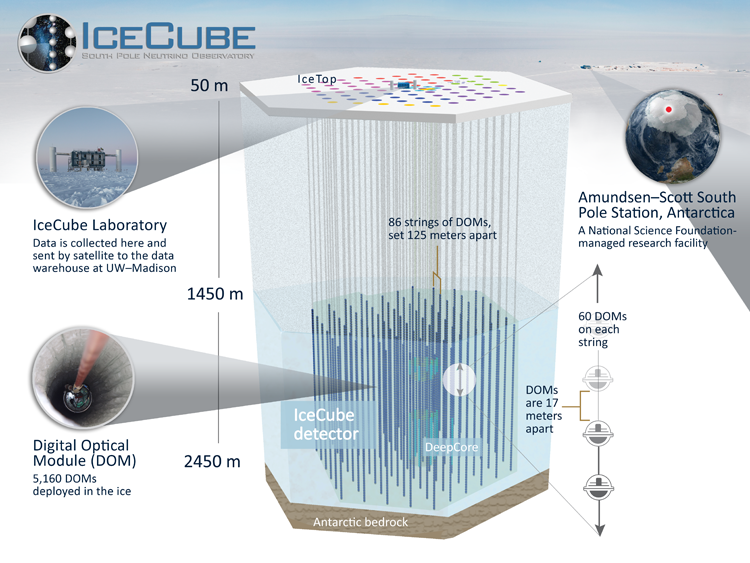
\includegraphics[width=0.7\textwidth]{icecube_detector_sm.png}
\caption{Diagram of the location and layout of the ICECUBE Observatory.}
\label{fig:ICECUBE}
\end{figure}


One of the challenges in high energy astrophysics is attributing a source to the detected arrival direction. Narrowing down the type of sources producing the neutrinos would greatly help in determining which catalogue to concentrate on when doing source searches. The current method uses a likelihood function to determine the probability of events being attributed to a set of sources. Each event is assumed to be independent. The basis of the likelihood function can be written as:
\begin{equation}
\mathcal{L} = \prod_{\mathrm{i}} \sum_{\mathrm{j}} S_{\mathrm{i}}(\mathrm{i} - \mathrm{j})
\end{equation}
Where i is the neutrino event, j is the source and $S$(i-j) is a function that would describe the probability that an event i is associated with a source j.


Our hypothesis is that there could be unique features in the arrival direction Sky Maps that can be used to determine or put limits on the number of sources producing neutrinos. We would like to investigate the usability of machine learning algorithms to test our hypothesis. The end goal would be to put limits on the number of observable sources that could produce the measured ICECUBE neutrino sky map.


We can already generate sky maps from simulations using different numbers of neutrino sources. The simulations use models of our best understandings of galaxy and star formations. After generating the sky maps, we would like to find a way to classify features and this is where we would like to include the machine learning algorithms. Our current thought is a harmonic scan and fit for as high order functions as possible. We are aware one of the challenges will be to have enough simulated data for the training set and the test set. After using the simulated data as a training data set, we can then test our hypothesis using the measured ICECUBE neutrino sky map to see what number range of sources the algorithm determines.


%\begin{figure}[!htp]
%\centering
%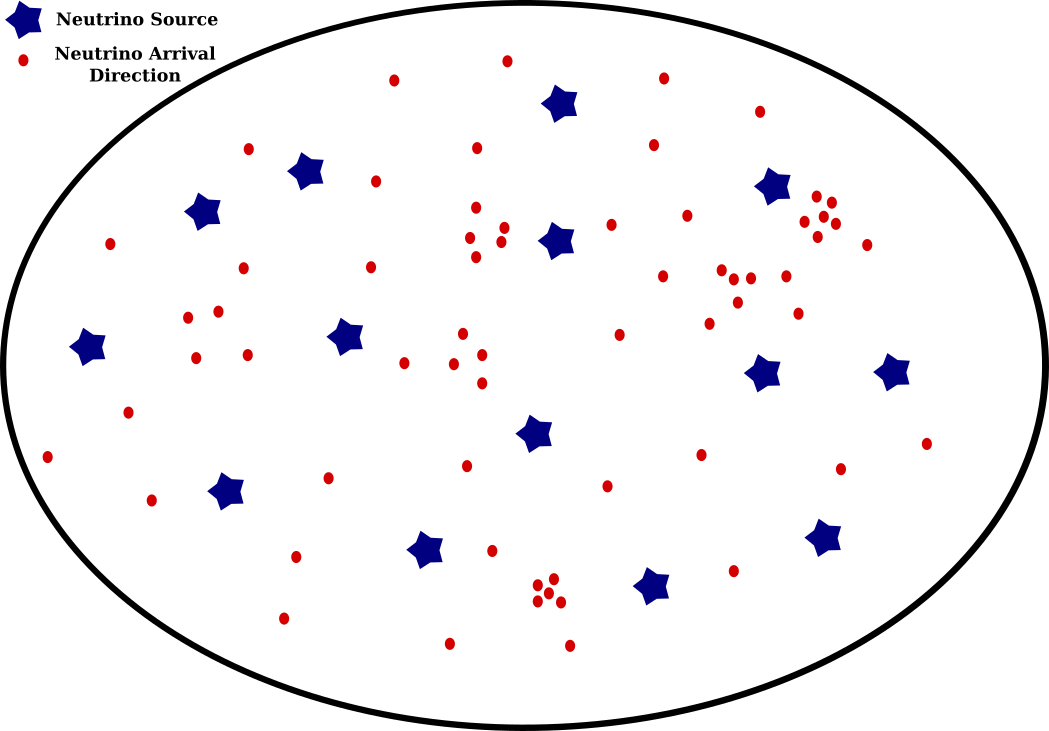
\includegraphics[width=0.6\textwidth]{MockNeutrinoMap.png}
%\caption{Diagrammatic example of how sources and arrival directions
%of neutrinos could be arranged over a sky map. Blue stars represent a neutrino source and red dots represent arrival directions.}
%\label{fig:SourceEventEx}
%\end{figure}


\end{document}

